\documentclass[11pt]{article}


\usepackage[problem]{handout}
\usepackage{alltt}
\usepackage{program}
\usepackage{hyperref}
\usepackage{graphicx}
\usepackage{pict2e}

\setlength{\unitlength}{2pt}

\newcommand{\ie}{{i.e.}}

\class{CompSci 351/CompSt 751: Data Structures \& Algorithms}
\period{Spring 2025}
\title[Homework \#3]{Homework \#3\\ 
\textbf{due Monday, February 10, 10pm}}

\begin{document}
\maketitle
In this homework, 
you will implement and then use a collection
class with an interface from Java's library collection system.
The collection will use the same data structure as Homework \#2
(``dynamic array''), this time for the \textsf{Collection} ADT rather than the
\textsf{Sequence} ADT.

Use this link to accept the assignment:
\begin{quote}
\url{INVITE_LINK}
\end{quote}

\section{Concepts}

In this week, you will work with several concepts that don't have
their own chapter in the textbook.

\subsection{Interfaces}

A Java ``interface'' is a special kind of ``abstract class.''
A Java \emph{interface} specifies a set of (public) operations
(``methods'' in Java) that an ADT
might be expected to implement.  An ADT implementation signals its
adherence to the interface by adding ``\texttt{implements $I$}'' 
to the class header, where
$I$ is the name of the interface.
Some interfaces don't mention any methods; 
rather they are \emph{marker} interfaces that 
mark the willingness of the class to satisfy certain properties.

Some of the Java standard interfaces that we will be using in this course are listed here:
\begin{description}
\item[\texttt{Cloneable}] A marker interface for classes that permit the built-in 
\verb|Object#clone()| method to make a shallow copy.
\item[\texttt{Comparable<T>}] These classes 
implement a \texttt{compareTo} method taking a parameter of type \texttt{T}.
\item[\texttt{Iterator<T>}] These are iterator objects.
\item[\texttt{Iterable<T>}] These classes will provide an
  \texttt{iterator()} method returning an iterator.
\item[\texttt{Collection<T>}] These are classes that provide all the collection methods 
(see below for more).
\end{description}

A Java variable (field, parameter or local) may have an interface as a
type.  Of course the variable is \emph{not} an instance of this type,
since interfaces are abstract---they don't provide any implementation.
Instead they are instances of some class that implements the interface.
In Java, it is considered better to use interfaces for the type of
variables or method returns instead of concrete classes since it makes
the program more general.

%In this assignment, you will need to use
%an interface called \verb|ActionListener| and
%one ``generic'' interface both described later.

\subsection{Generics}

Many of the library classes are \emph{generic} so that they work with
different reference types (e.g., classes).
In this homework, we will work with several generic interfaces and
classes.  If you fail to give the actual generic type parameter
(inside angle brackets, e.g., \verb|List<String>|), Eclipse will
warn you that you are using ``raw types.'' Raw types are not allowed
for CS~351 homeworks, so make sure to take heed of the warnings.

\subsection{Collection ADT}

The Java standard collection framework includes an interface
\texttt{Collection} with a number of methods.  See the textbook
Figure 5.7, page 301 (3rd.\ ed.\ Fig.\ 5.6, p.\ 290), or look at 
\href{https://docs.oracle.com/javase/8/docs/api/java/util/Collection.html}{the online documentation}.

For this assignment, you will write a class that implements
the standard Java Collection interface which has the following
methods (in addition to ones every object has):
\begin{description}
    \item[size()] Return the number of elements in the collection.
    \item[isEmpty()] Return whether the collection is empty.
    \item[contains(Object)] Return whether the collection contains the parameter.
    \item[iterator()] Return an iterator over the elements.
    \item[toArray()] Return an array of all elements.
    \item[add($E$)] Add an element to the collection and return true.
    \item[remove(Object)] Remove an element from the collection and
      return true, or return false if it was not found.
    \item[containsAll(Collection)] Return true if every element in the
      parameter is also present in this collection.
    \item[addAll(Collection)] Add all the elements from the parameter
      to this collection, returning true if anything was added.
    \item[removeAll(Collection)] Remove all the elements in the parameter
      from this collection, returning true if anything was removed.
    \item[retainAll(Collection)] Remove all the elements in this
      collection that do not also occur in the parameter; returning
      true if anything was removed.
    \item[clear()] Remove everything from the collection.
\end{description}
But it's a lot of work to implement all these methods so Java provides a class \texttt{AbstractCollection} that implements all but two of these methods.
You should have your class extend \texttt{AbstractCollection}.
See \href
{https://docs.oracle.com/javase/8/docs/api/java/util/AbstractCollection.html}{the online documentation}.

When you implement a class that inherits from an abstract class
like \texttt{AbstractCollection}, you must decide which methods to override.
Some reasons to override include:
\begin{enumerate}
\item The abstract class does not provide an implementation
  for this method, so that Java \emph{requires} that we
  override/implement the method.  Keyword: \texttt{required}
\item The provided implementation is incorrect.  For example, it may
  simply throws an exception indicating that the method is not
  \emph{really} implemented.
(Immutable classes typically use this approach for all methods that
  can modify the collection.)
  Keyword: \texttt{implementation}
\item The provided implementation is logically correct, but
  inefficient for your data structure.
  Keyword: \texttt{efficiency}
\item The inherited implementation needs to be added to in some way.  Keyword: \texttt{decorate} (This kind of overriding is used only by \texttt{clone} for this assignment.)
\end{enumerate}\texttt{AbstractCollection}.
See \href
{https://docs.oracle.com/javase/8/docs/api/java/util/AbstractCollection.html}{the
  online documentation}. 

When you implement a class that inherits from an abstract class
like \texttt{AbstractCollection}, you must decide which methods to override.
Some reasons to override include:
\begin{enumerate}
\item The abstract class does not provide an implementation
  for this method, so that Java \emph{requires} that we
  override/implement the method.  Keyword: \texttt{required}
\item The provided implementation is inefficient for your data
  structure.
  Keyword: \texttt{efficiency}
\item The provided implementation is incorrect.  For example, the \texttt{add} method of \texttt{AbstractCollection}
  simply throws an exception indicating that the method is not
  \emph{really} implemented.
(Immutable classes typically use this approach for all methods that
  can modify the collection.)
  A mutable collection will need to override this implementation.
  Keyword: \texttt{implementation}
\item The inherited implementation needs to be added to in some way.  Keyword: \texttt{decorate} (This kind of overriding is not used in this assignment.)
\end{enumerate}
If none of these apply, you should refrain from overriding.
Please comment all overridings with the keyword,
(e.g. ``\texttt{@Override //
  efficiency}'').

\subsection{Iterators}

\texttt{Collection}s, as well as some other classes, provide iterators, which
are an interface allowing access to each element, one-at-a-time, and once each.
We implemented something similar as part of the \texttt{Sequence} ADT,
but iterators are more powerful than such ``cursors.''
The big advantages are (1) that one can have multiple
iterators (whereas there's just one cursor for each \textsf{Sequence})
and (2) then changing the state of an iterator (e.g., advancing it) does not affect the collection itself.
But since iterators are separate objects from the collections, if the
collection changes, the iterator can go ``stale.''  Implementations
try to prevent the usage of stale iterators, throwing an instance of
\texttt{ConcurrentModificationException} but the checks are not
foolproof.  

Java's iterators have the following methods:
\begin{description}
\item[hasNext()] Return true if there are elements that have not
yet been accessed by this iterator.
\item[next()] Advances the iterator, accessing and returning
  an element that had not yet been accessed (now the current element).
  If there is no such element (in which case \verb|hasNext()| should have returned
  false), then throw an instance of \verb|NoSuchElementException|.
\item[remove()] Remove the current element (the one \emph{previously} returned by
  \verb|next()|). If \texttt{next()} has not yet been called, or if
  the last accessed element has already been removed, then this method throws an
  \texttt{IllegalStateException}, since there is no current element.
\end{description}
Each iterator moves separately through the container. Our iterator is a nested
class, so it is able to access private fields and methods of the collection.

The \verb|Iterator| interface is generic; the type of the elements
in the collection needs to be specified.
To access all the elements of a collection, and decide whether to
delete them, one can write:
\begin{quote}
\begin{program}
for (Iterator<$T$> it = $c$.iterator(); it.hasNext();) \{
   $T$ x = it.next();
   if (\w{we don't want element x any more}) it.remove();
\}
\end{program}
\end{quote}
In this assignment, we will be using iterators specifically on
\texttt{HexTile} objects.

Java has a special syntax of ``enhanced'' for-loops to make it easy to use
iterators.  The shortcut:
\begin{quote}
\begin{program}
for ($T$ $x$ : $c$) \{
   ...
\}
\end{program}
\end{quote}
is short for
\begin{quote}
\begin{program}
for (Iterator<$T$> secret = $c$.iterator(); secret.hasNext();) \{
   final $T$ $x$ = secret.next();
   ...
\}
\end{program}
\end{quote}

\subsection{Fail-Fast Iterators}

When using standard Java collections,
iterators become ``stale'' if the collection changes, except by using
the iterator's own \verb|remove| method.  (This does not happen with
cursors, because the ADT has more control over its cursors.)
It is not legal to
use a stale iterator for anything, even calling \verb|hasNext|.
In other words, if you request an iterator and later add an element to
the collection, then you are not allowed to use the iterator again.
If you want an iterator, you must request a new one.

Implementors of Java's standard 
collections are encouraged to provide \emph{fail-fast}
implementations of iterators which ``usually'' throw an exception
(an instance of \textsf{ConcurrentModificationException})
when a stale iterator is used.

Typically, this ability is handled by adding an integer version stamp to every
collection and iterator.  The version should be incremented inside \emph{every method} that
modifies the number of elements in the collection (or moves them around).  If an iterator
notices that the version doesn't 
match, it throws the required exception before performing any method.
This is \emph{not} part of the invariant: if the invariant fails, it
is because the ADT implementation contained a bug; if the version stamp doesn't match it
is because the ADT was misused. Therefore, if the versions don't
match, do not check anything in the invariant checker.

The iterator version only changes if the collection was changed under
its control (i.e., using \verb|remove|).

\subsection{Nested classes}

A (non-static)
nested class is interesting: it is considered to be ``inside of'' the
object in which it was created and thus has access to all the
(private) fields and (private) methods as if they were its own.
This is not inheritance: it doesn't actually get any fields or methods
from the surrounding class, but it \emph{can} access them.
It is even more confusing if the nested class extends some other
class.  But we won't do that for this assignment.

Nested classes are often used to implement iterators since an iterator
needs access to private internals of the collection class.
%Nested classes (and anonymous classes) are also used to implement
%listeners, if you don't always want \verb|this| to be its own listener.
Within the iterator, you can use the fields of the outer class directly.
If there are two fields or methods with the same name in the outer and inner classes,
you can refer to the one in the outer class by the syntax 
\emph{OuterClassName.this.name}.
For example, in this homework, the iterator's invariant checker will
need to call (not assert!) the \verb|wellFormed| in the outer class
(instead of the one within the iterator), by including the call
\verb|HexTileCollection.this.wellFormed()|.

%\subsection{Variable-Arity Parameters}%
%
%You may have noticed that the driver for Homework~\#3 had a method
%whose parameter had type \verb|HexTile...| and was called with a
%variable number of parameters.  Java supports variable arity methods
%by implicitly creating an array around them and passing the array.
%Thus inside the method body, the variable-arity paranmeters can be
%accessed using normal array operations.

%\subsection{Event Handlers}
%
%With Java's graphics model, events are reacted to, rather than
%detected.  In other words, rather than repeatedly asking ``Did someone
%click my window?'' a Java application program will say ``when someone
%clicks my window, let me know.''  The application program will call 
%\verb|add|$X$\verb|Listener| on the window or applet 
%from which it wants to receive events, where $X$ is the kind of event.
%Then the general event system will
%call a method when the window is clicked.  The object to be notified
%must implement the required interface.  
%
%% One can use anonymous classes as event handlers, but in this homework,
%% we will simply have the applet itself implement the event handling interface And
%% the required methods.
%% In the case of mouse clicking,
%% the interface is named \verb|MouseListener|.  If one is only interested
%% in clicking (as for this assignment), all the required methods can have empty
%% bodies except for the method named \verb|mouseClicked|.
%
%\subsection{Anonymous classes}
%
%This week, we will work with the 
%``action listener'' and ``mouse listener'' interfaces.  The former is simpler:
%\begin{verbatim}
%public interface ActionListener {
%  public void actionPerformed(ActionEvent e);
%}
%\end{verbatim}
%One could define a class that implemented this interface and then
%create an instance of it:
%\begin{verbatim}
%public class MyActionListener implements ActionListener {
%  public void actionPerformed(ActionEvent e) {
%    // do something
%  }
%}
%...
%        new MyActionListener()
%\end{verbatim}
%But frequently, we don't really care what the name of the class is, we only want
%to make an instance of it.  In that case we can create an instance
%of an \emph{anonymous class} using the following syntax:
%\begin{quote}
%\begin{verbatim}
%new ActionListener() {
%  public void actionPerformed(ActionEvent e) {
%    // do something
%  }
%}
%\end{verbatim}
%\end{quote}
%This \emph{looks} as if we are creating an instance of the interface,
%but actually we are creating an instance of a class that is never given
%a (visible) name.  The anonymous class implements the interface and
%defines the method \verb|actionPerformed|.
%
%This syntax can be used to create instances of anonymous subclasses
%of normal classes too.  For instance, the class \texttt{MouseAdapter}
%implements the \texttt{MouseListener} interface with methods that do
%nothing.  One can make an instance that does something different for
%one or more of the methods by using the anonymous class syntax:
%\begin{quote}
%\begin{verbatim}
%this.addMouseListener(new MouseAdapter() {
%    @Override
%    public void mouseClicked(MouseEvent e) { ... }
%});
%\end{verbatim}
%\end{quote}
%%\textbf{NB}: To distinguish between a double-click and a single-click, use
%%\verb|getClickCount| on the mouse event object.  A double click
%%is always preceded by a single click in the same location.
%
%\noindent
%\textbf{NB:} The solution uses anonymous classes for the mouse
%listener and for the action listeners on the terrain buttons.
%
%\begin{latexonly}
%\begin{ignore}
%\section{Concurrent Programming without Race Conditions}
%
%Our animation programs are multi-threaded programs because the
%timer/animation thread is different from the thread that handles
%updating the screen.  Programming for this model requires some careful
%work.  We were sloppy in the last homework, but this homework, you
%will need to be careful to follow these rules:
%\begin{itemize}
%\item If a mutable field can be accessed in multiple threads, it
%  should be marked ``volatile''\footnote{%
%Or be protected by a synchronization lock, but that is too complicated
%for us in CS 351.  CS 552 and 537 have more information on synchronization.}.
%\item You can't change library classes.
%\end{itemize}
%One important consequence of these two simple rules is that a mutable
%collection (instance of library class) must not be accessed in multiple
%threads.  The simple solution is to make sure all shared collections
%are \emph{immutable}: they never change.  
%
%In particular, the
%collection of blocks used in the simulation should never change.
%How then can one add or remove blocks?  There's a trick!  We make a
%\emph{new} collection that is a copy of the list of blocks, make
%changes to it (in one thread) and then install it as the (immutable!) list of
%blocks being simulated.  The field that holds the list is mutable
%(and will be marked ``volatile'').
%
%\subsection{Mutable Data Classes}
%
%If a class consists of fields with setters and getters, we call
%it a ``data class.'' Such a class isn't a classic ADT, but just a way to stick
%things together.  Use getters and setters rather than making the
%fields public (a terrible idea) does have certain advantages.
%In particular they can be overridden by subclasses.  We may see 
%examples of this in the second half of this course.
%A mutable data class doesn't have fixed values and thus it usually best practice
%to \emph{not} override \texttt{equals} or \texttt{hashCode}.
%
%\section{Conversions from String}
%
%In our first week, we implemented \verb|toString()| methods
%for getting a string version of the ADTs.  The reverse methods enables
%ADT values to be written to text files and then read back in.
%All three of our Homework \#~1 ADTs need static \verb|fromString|
%methods;
%we have implemented the most complex one for you: \verb|Time.fromString|.
%We provide test cases for these conversions.
%
%You need to write the following string conversion methods:
%\begin{description}
%\item[Duration\#fromString(String)] (static)
%   Convert a duration string back into a duration.
%\item[Period\#fromString(String)] (static)
%   Convert a period string back into a period.
%\end{description}
%These methods should throw an instance of
%\verb|edu.uwm.cs351.util.FormatException| if an error in the string is
%detected.  In particular, a \verb|NumberFormatException| must be
%caught and converted into a \verb|FormatException| (there is a
%constructor for this purpose).
%\end{ignore}
%\end{latexonly}


\section{Concerning the \texttt{HexTileCollection} class}

In the last homework, you implemented a \textsf{Sequence} ADT
(specifically for hex tile objects) with a dynamic array data structure.
For this assignment you will implement a \textsf{Collection} ADT,
using \texttt{AbstractCollection}.
You need to implement the \texttt{wellFormed} method for this class;
it will be simpler than what you wrote for Homework \#2 because we
have only the dynamic arrays, not the cursor.

You will need to override some
methods from the superclass/interface.  Only override the ones you
need to override for one of the three reasons given above, and
repeated here: it is \emph{required} by Java; we need to provide a
more \emph{efficient} implementation, or for \emph{implementation}
purposes (because the overridden implementation does the wrong thing).

For the \textsf{Collection} interface, where an element goes if it is
added is not specified, and indeed the ``add'' operation is optional to define.
But our \texttt{HexTileCollection} ADT, \emph{does} define \texttt{add}:
it places the argument hex tile at the end of the collection, and then
returns ``true.''

Iteration over this collection must have
fail-fast semantics.  To do so, the main class should have a field
named ``version'' that is incremented each time the number of elements
is changed. Then the iterator will remember the version it was created
for in a local field and then each public iterator method will check if
there is a version discrepancy, in which case they throw an instance
of \texttt{ConcurrentModificationException}.  The \texttt{remove}
method will (of course) change the collection version and thus should
also change the iterator's version, because it is still in sync with
the collection.

\subsection{Concerning the data structure of the iterator}

The iterator should use the following data structure.
It's more complicated than the cursor implementation because we need
to make sure someone doesn't call \texttt{remove} twice in a row:
\begin{description}
  \item[currentIndex] The current index (index of the part most
    recently returned by \texttt{next()}), that would be removed by
    \texttt{remove()}.   If there is no such element, then it should be
    the index of the previous element (initially -1).
  \item[isCurrent] Whether there is an element at the current index
    that can be removed.
  \item[colVersion] The version of the collection that this iterator is
    set up to work for.
\end{description}
You need to complete the \texttt{wellFormed} method.  The first thing
it should do is to check the outer invariant using the syntax
\begin{quote}
  \texttt{HexTileCollection.this.wellFormed()}
\end{quote}
If the outer invariant fails, the iterator should return false without
reporting anything in addition.

Then, perhaps unintuitively, the invariant checker should
\emph{succeed} if the 
version doesn't match.  That is because the invariant is used to
protect against errors in the implementation of the collection class
(or its iterator).  If the version doesn't match then it's not the
fault of the implementer of the collection class; it's the fault of
the user.  In such a case, the version could be very stale, so we
don't check anything and blithely return ``true.''

You should then check:
\begin{enumerate}
  \item The \texttt{currentIndex} field is a valid index in the dynamic array,
    or equal to -1.
  \item If \texttt{isCurrent} is true, the index must be a valid
    index (-1 is not allowed).
\end{enumerate}
As usual, if no problems are found, we return true.

\subsection{Note on debugging collection classes}

The Eclipse debugger has an option to ``Show Logical Structure''
\begin{quote}
  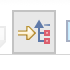
\includegraphics{show-logical-structure}
\end{quote}
that you \emph{must} make sure is turned off (not boxed/highlighted)
when debugging \texttt{HexTileCollection} (or any collection class you
implement for this course).
Otherwise, the debugger will not show you the fields of the class,
but instead use the iterator methods to show what elements are in the collection.
But if your iterator is not working (and that is one big reason why you would be debugging it!), 
the display will not work.

\subsection{Concerning the addition to the \texttt{HexTile} class}

We are adding a new method to \texttt{HexTile}:
\begin{description}
  \item[fromString(s)] Convert a string to a hex tile.  The string
    must have the form of a terrain string concatenated to a hex
    coordinate string.
\end{description}

\subsection{Concerning the \texttt{Demo} class}

Once the \texttt{HexTileCollection} class is working, you need to
modify the \texttt{Demo} class 
to use \texttt{HexTileCollection}.
We provide a most of the implementation---you will need to implement
what is remaining.  You may wish to refer to the code for
\verb|Demo| in the solution to Homework \#2.  The code should work the same
as in that homework, but you now need to use the iterator instead of changing the ADT state with \texttt{advance()}.
You also need to use the newly added \texttt{fromString} method in the \texttt{HexTile} class.
% Don't add new public methods to the \texttt{} class to match the old API!
We recommend using the ''enhanced'' for-loop syntax mentioned above to keep things looking neat, but remember that behind the scenes it is using your own
iterator implementation!


\section{What You Need To Do}

Here are the recommended steps for this assignment.  After each step,
and after each session.
make sure to commit (and push if possible) your code.
\begin{enumerate}
\item In the starting repository, there is a very limited skeleton
  file for \texttt{HexTileCollection}.  Add declarations so as to remove
  all compiler errors.  In particular, compiler error in the Spy
  must be handled by fixing the main class.  For instance, the Spy
  assumes certain names for the fields---conform to these
  assumptions.  Do not edit the Spy in
  any circumstances---even if Eclipse suggests it!  If you find that
  somehow you changed the Spy, see a TA to get the Spy restored.
  
  You will also need to add declarations so that the test
  classes have no compilers error too.
  
  If a method needs to be added, then add a \emph{stub}: a
  compiler-acceptable definition that does nothing interesting, for
  example, returning \texttt{null} if some return object is
  required.
  
  You must ensure that you have no ``raw'' type warnings.  These
  indicate that you neglected to give the element type of a
  collection or iterator.
  
\item
  Then implement the \emph{two} \texttt{wellFormed} methods (for the
  main class and for the iterator) and check that your
  implementations pass the invariant tests: \texttt{TestInvariant}.
  
\item
  Next unlock all remaining tests using \texttt{UnlockTest}: make
  sure that you add the generated ``tst'' file to \textsf{git}.
  
\item
  Then complete all the stubs in the main class.  Check that you
  pass the tests in \texttt{TestHexTileCollection} (inherited from
  abstract test class \texttt{TestCollection}) up through
  \texttt{test06}.  (You can ignore the \texttt{test9}$n$ tests until
  late in the process.)
  
\item
  Then implement the iterator (except for removal) and make sure you can pass all the
  tests through \texttt{test35}.
  
\item Then implement iterator remove and check that your code now
  passes all the tests in \texttt{TestHexTileCollection} except for
  \texttt{test9}$n$.

\item Now implement \texttt{HexTile.fromString} and pass the remaining tests.
  
\item Use random testing to make sure you haven't worked around
  the tests with special cases.  Once you pass random testing, it
  is time to check efficiency.
  
\item Test that your algorithms are efficient with
  \texttt{TestEfficiency}.  Most people's code will fail at least one, the
  first time the test is run.  Fix the code so that passes efficiency
  testing.

\item Then re-run \texttt{TestHexTileCollection} and random testing to
  make sure that you didn't mess up
  a special case when handling efficiency.  It is a frequent occurrence
  for random testing to fail at this point, even though it was passing
  before.  Analyze the test that random testing gives you to find
  where your code is handling a special case incorrectly.
  
\item Once all the tests are passing, move on to update the
  implementation of \texttt{Demo} this time to use the collection
  ADT.  This exercise ensures that you are able to \emph{use} the
  collection ADT to accomplish some non-trivial tasks.
\end{enumerate}  

\section{Hints}

New to this homework assignment are efficiency tests.
Efficiency tests often fail in different ways than normal tests.  Of
course, you can have a normal failure, but the interesting failure is
when it takes a long time.  Typically the code is not in an infinite
loop (a very basic efficiency problem you may have encountered in
earlier courses) but just is not using the appropriate algorithm to
finish the task in a reasonable length of time.  There's nothing
``wrong'' with what the code is doing step by step, but it just
takes too long.

Furthermore, the fact that code takes a long time to run usually makes
the typical ways of using a debugger (e.g., stopping the code at certain
breakpoints and checking the values of variables) ineffective,
because they simply take too long.
Rather you should use the debugger, or even print statements to see if
code reaches certain points in the test.\footnote{If you edit the
  tests to add print statements, make sure to revert the changes, for
  example using ``Replace With'' the \texttt{HEAD} version), before
  committing the code.}

It is even more important to analyze the test to see what it is doing:
what is it doing a millions times?  Is that operation a constant-time?
(Or at most log-time, as we shall see in later homework assignments).
When you get stuck, post a question on Piazza that includes your analysis
of what the test is doing: why is the test right to expect that
operation should be fast?  (Or why do you disagree, that the operation
cannot be fast?) Look for loops in the code that should be constant time.

Here are some hints for this week's efficiency tests:
\begin{description}
\item[test0] Why should \texttt{add} be constant time (on average)?
\item[test3] How much is needed to initialize an iterator?
\item[test4] How much work is needed to do \texttt{next}?
\item[test5] How is \texttt{clear} implemented by default?  Can you
  do better?
\end{description}

\section{Objectives}

In doing this homework, it is intended that the student will learn
\begin{itemize}
\item to declare that a class implements an interface,
\item to use the fact that a class implements an interface,
\item to use generic library classes,
% \item to use \texttt{ArrayList} to build a two-dimensional data
%  structure,
\item to implement a collection class, and when to override
  methods,
\item to use iterators, in normal ``for'' loops and also
  ``for-each'' loops,
\item when an iterator may be stale,
\item to implement a fail-fast iterator,
\item how to use a data structure to enable efficiency
  implementations,
\item to implement a static \texttt{FromString} method,
  and
\item how to diagnose elementary efficiency problems.
\end{itemize}
  
\end{document}

% LocalWords:  CS unenrolls ItemType int ADT turnin cc README href html STL cpp





% LocalWords:  ADTs destructor const CLASSHOME Makefile ArrayList HexTile java
% LocalWords:  hasNext NoSuchElementException IllegalStateException src getRGB
% LocalWords:  ConcurrentModificationException MouseListener mouseClicked AFS
% LocalWords:  getClickCount ActionListener ArrayCollection actionPerformed
% LocalWords:  fromString fromString hexString NumberFormatException BlockSeq
% LocalWords:  FormatException CollisionApplet isEmpty toArray addAll
%%  LocalWords:  containsAll removeAll retainAll Microsystems boolean
%%  LocalWords:  AbstractCollection Implementors wellFormed isCurrent
%%  LocalWords:  currentIndex calledNext ParticleCollection Cloneable
%%  LocalWords:  ManyParticles ParticleSeq compareTo Iterable tst
% LocalWords:  HexTileCollection superclass colVersion TestInvariant
% LocalWords:  UnlockTest TestHexTileCollection TestCollection
% LocalWords:  TestEfficiency
